\documentclass{book}

\usepackage{amsmath}
\usepackage{amssymb}
\usepackage{chemfig}
\usepackage{mathtools}
\usepackage{listings}
\usepackage{color}
\usepackage{wrapfig}
\usepackage{float}
\usepackage{caption}
\usepackage{fourier}
\usepackage{subcaption}
\usepackage{multicol}
\usepackage{paralist}
\usepackage{tcolorbox}
\usepackage{braket}
\usepackage[framemethod=TikZ]{mdframed}
\usepackage[english]{babel}
\usepackage[utf8x]{inputenc}
\usepackage[colorinlistoftodos]{todonotes}
\usepackage{esint}

\title{College Notes}
\date{2019-01-01}
\author{Animesh Sinha}


\newcounter{theo}[section]\setcounter{theo}{0}
\renewcommand{\thetheo}{\arabic{section}.\arabic{theo}}
\newenvironment{theorem}[2][]{%
\refstepcounter{theo}%
\ifstrempty{#1}%
{\mdfsetup{%
frametitle={%
\tikz[baseline=(current bounding box.east),outer sep=0pt]
\node[anchor=east,rectangle,fill=blue!20]
{\strut Theorem~\thetheo};}}
}%
{\mdfsetup{%
frametitle={%
\tikz[baseline=(current bounding box.east),outer sep=0pt]
\node[anchor=east,rectangle,fill=blue!20]
{\strut Theorem~\thetheo:~#1};}}%
}%
\mdfsetup{innertopmargin=10pt,linecolor=blue!20,%
linewidth=2pt,topline=true,%
frametitleaboveskip=\dimexpr-\ht\strutbox\relax
}
\begin{mdframed}[]\relax%
\label{#2}}{\end{mdframed}}


\newcounter{trk}[section]\setcounter{trk}{0}
\renewcommand{\thetrk}{\arabic{section}.\arabic{trk}}
\newenvironment{trick}[2][]{%
\refstepcounter{trk}%
\ifstrempty{#1}%
{\mdfsetup{%
frametitle={%
\tikz[baseline=(current bounding box.east),outer sep=0pt]
\node[anchor=east,rectangle,fill=blue!20]
{\strut Trick~\thetrk};}}
}%
{\mdfsetup{%
frametitle={%
\tikz[baseline=(current bounding box.east),outer sep=0pt]
\node[anchor=east,rectangle,fill=blue!20]
{\strut Trick~\thetheo:~#1};}}%
}%
\mdfsetup{innertopmargin=10pt,linecolor=blue!20,%
linewidth=2pt,topline=true,%
frametitleaboveskip=\dimexpr-\ht\strutbox\relax
}
\begin{mdframed}[]\relax%
\label{#2}}{\end{mdframed}}


\newcounter{prf}[section]\setcounter{prf}{0}
\renewcommand{\theprf}{\arabic{section}.\arabic{prf}}
\newenvironment{proof}[2][]{%
\refstepcounter{prf}%
\ifstrempty{#1}%
{\mdfsetup{%
frametitle={%
\tikz[baseline=(current bounding box.east),outer sep=0pt]
\node[anchor=east,rectangle,fill=red!20]
{\strut Proof~\theprf};}}
}%
{\mdfsetup{%
frametitle={%
\tikz[baseline=(current bounding box.east),outer sep=0pt]
\node[anchor=east,rectangle,fill=red!20]
{\strut Proof~\thetheo:~#1};}}%
}%
\mdfsetup{innertopmargin=10pt,linecolor=red!20,%
linewidth=2pt,topline=true,%
frametitleaboveskip=\dimexpr-\ht\strutbox\relax
}
\begin{mdframed}[]\relax%
\label{#2}}{\end{mdframed}}


\newcounter{exm}[section]\setcounter{exm}{0}
\renewcommand{\theexm}{\arabic{section}.\arabic{exm}}
\newenvironment{example}[2][]{%
\refstepcounter{exm}%
\ifstrempty{#1}%
{\mdfsetup{%
frametitle={%
\tikz[baseline=(current bounding box.east),outer sep=0pt]
\node[anchor=east,rectangle,fill=green!20]
{\strut Example~\theexm};}}
}%
{\mdfsetup{%
frametitle={%
\tikz[baseline=(current bounding box.east),outer sep=0pt]
\node[anchor=east,rectangle,fill=green!20]
{\strut Example~\thetheo:~#1};}}%
}%
\mdfsetup{innertopmargin=10pt,linecolor=green!20,%
linewidth=2pt,topline=true,%
frametitleaboveskip=\dimexpr-\ht\strutbox\relax
}
\begin{mdframed}[]\relax%
\label{#2}}{\end{mdframed}}


\newcounter{def}[section]\setcounter{def}{0}
\renewcommand{\thedef}{\arabic{section}.\arabic{def}}
\newenvironment{definition}[2][]{%
\refstepcounter{def}%
\ifstrempty{#1}%
{\mdfsetup{%
frametitle={%
\tikz[baseline=(current bounding box.east),outer sep=0pt]
\node[anchor=east,rectangle,fill=yellow!20]
{\strut Definition~\thedef};}}
}%
{\mdfsetup{%
frametitle={%
\tikz[baseline=(current bounding box.east),outer sep=0pt]
\node[anchor=east,rectangle,fill=yellow!20]
{\strut Definition~\thetheo:~#1};}}%
}%
\mdfsetup{innertopmargin=10pt,linecolor=yellow!20,%
linewidth=2pt,topline=true,%
frametitleaboveskip=\dimexpr-\ht\strutbox\relax
}
\begin{mdframed}[]\relax%
\label{#2}}{\end{mdframed}}


\newcounter{note}[section]\setcounter{note}{0}
\renewcommand{\thenote}{\arabic{section}.\arabic{note}}
\newenvironment{note}[2][]{%
\refstepcounter{note}%
\ifstrempty{#1}%
{\mdfsetup{%
frametitle={%
\tikz[baseline=(current bounding box.east),outer sep=0pt]
\node[anchor=east,rectangle,fill=pink!20]
{\strut Note~\thenote};}}
}%
{\mdfsetup{%
frametitle={%
\tikz[baseline=(current bounding box.east),outer sep=0pt]
\node[anchor=east,rectangle,fill=pink!20]
{\strut Note~\thenote:~#1};}}%
}%
\mdfsetup{innertopmargin=10pt,linecolor=pink!20,%
linewidth=2pt,topline=true,%
frametitleaboveskip=\dimexpr-\ht\strutbox\relax
}
\begin{mdframed}[]\relax%
\label{#2}}{\end{mdframed}}



\let\cleardoublepage\clearpage


\begin{document}
\pagenumbering{arabic}


\begin{titlepage}
    \newcommand{\HRule}{\rule{\linewidth}{0.5mm}}
    \center
    \textsc{\LARGE International Institute of Information Technology, Hyderabad}\\[1.5cm]
    
\includegraphics[scale=1]{img/iiit-logo.jpeg}\\[0.5cm]
    \textsc{\Large First Year}\\[0.5cm]
    \textsc{\large Real Analysis, Digital Systems, Dicrete Mathematics, Computer Programming}\\[0.5cm] % Minor heading such as course title
    \HRule \\[0.4cm]
    { \huge \bfseries College Notes}\\[0.4cm]
    \HRule \\[1.5cm]
    \begin{minipage}{0.4\textwidth}
    \begin{flushleft} \large
    \emph{Author:} Animesh Sinha
    \end{flushleft}
    \end{minipage}\\[2cm]
    {\large \today}\\[2cm]
    \vfill
\end{titlepage}

\chapter{Particle Physics for Data Scientists}



\section{The Preliminaries}


\subsection{Problems with the standard model}

What makes us unhappy?
\begin{itemize}
  \item Matter and Antimatter inequivalence.
  \item 19 Arbitrary constants.
  \item Why is Gravity so weak.
\end{itemize}


\subsection{The Particles we want to detect}

\begin{figure}[H]
  \centering
  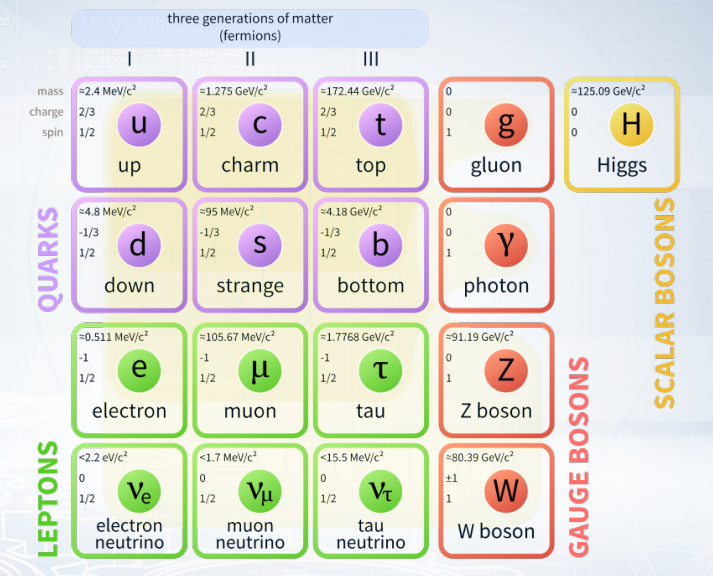
\includegraphics[width=0.4\linewidth]{img/hadron/particleid-list.png}
  \caption{List of Particles of different types}
  \label{fig:particleid-list}
\end{figure}

The following are types of particles we want to defect.
\begin{multicols}{3}
  \begin{itemize}
    \item muon
    \item kon
    \item pion
    \item proton
    \item electron
  \end{itemize}
\end{multicols}



\subsection{The Experiments in LHC}

There are 4 major detectors
\begin{itemize}
  \item ALICE (A Large Ion Collider Experiment) is a heavy-ion detector on the Large Hadron Collider (LHC) ring. It is designed to study the physics of strongly interacting matter at extreme energy densities, where a phase of matter called quark-gluon plasma forms.
  \item ATLAS (A Toroidal LHC ApparatuS) is one of two general-purpose detectors at the Large Hadron Collider (LHC). It investigates a wide range of physics, from the search for the Higgs boson to extra dimensions and particles that could make up dark matter. Although it has the same scientific goals as the CMS experiment, it uses different technical solutions and a different magnet-system design. It has a cylindrical structure and measures particles in all directions.
  \item CMS (Compact Muon Solenoid) is a general-purpose detector at the Large Hadron Collider (LHC). It has a broad physics programme ranging from studying the Standard Model (including the Higgs boson) to searching for extra dimensions and particles that could make up dark matter. Although it has the same scientific goals as the ATLAS experiment, it uses different technical solutions and a different magnet-system design.
  \item LHCb (Large Hadron Collider Beauty) experiment specializes in investigating the slight differences between matter and antimatter by studying a type of particle called the "beauty quark", or "b quark". It is a single arm forward spectrometer.
\end{itemize}

We smash bunches of protons ('events'), record the pixels ('hits'), reconstruct trajectories ('jets', 'showers', 'tracks'), and we perform Statistical analysis on them.

A Trigger System is a system that uses criteria to rapidly decide which events in a particle detector to keep when only a small fraction of the total can be recorded.


\subsection{Simulation Package}

\begin{itemize}
  \item http://www.genie-mc.org/
  \item http://home.thep.lu.se/Pythia/: Nutrino Simulations
  \item GEANT4: http://geant4.web.cern.ch/: Particles interacting with matter.
  \item FLUKA: http://www.fluka.org/fluka.php
\end{itemize}


\subsection{Feynman Diagrams}

\begin{figure}[H]
  \centering
  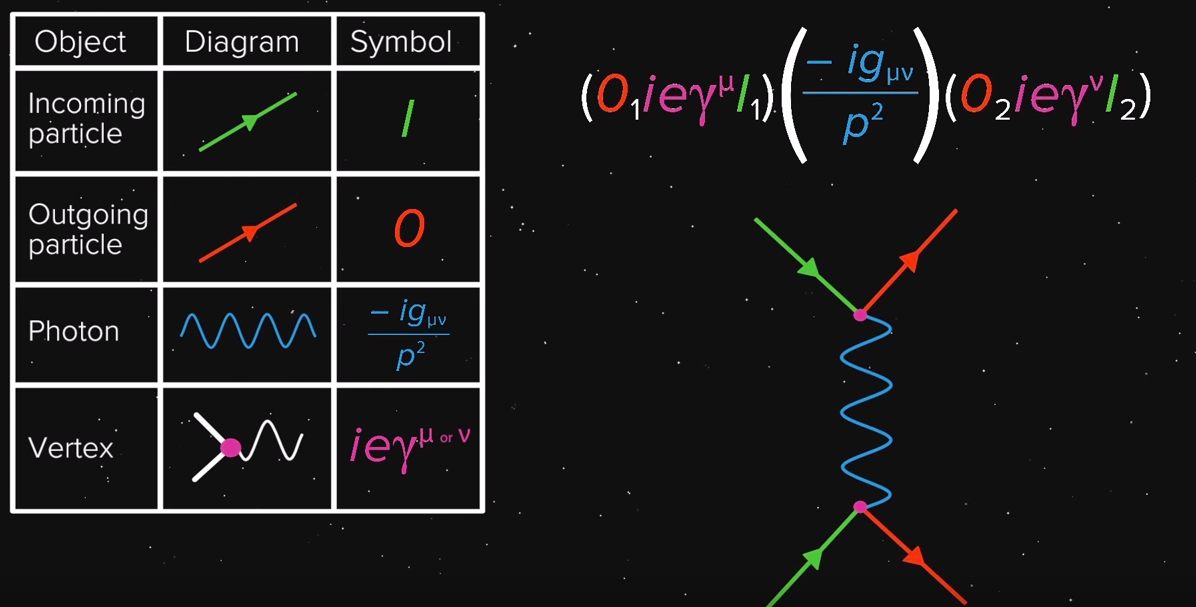
\includegraphics[width=0.8\linewidth]{img/hadron/preliminary-feynman-diagram.png}
  \caption{A Sample Feynman Diagram for scattering of Two electron by the transfer of one Photon}
  \label{fig:preliminary-feynman-diagram}
\end{figure}



\section{The Large Hadron Collider Setup}

\begin{figure}[H]
  \centering
  \begin{subfigure}[b]{0.5\textwidth}
    \centering
    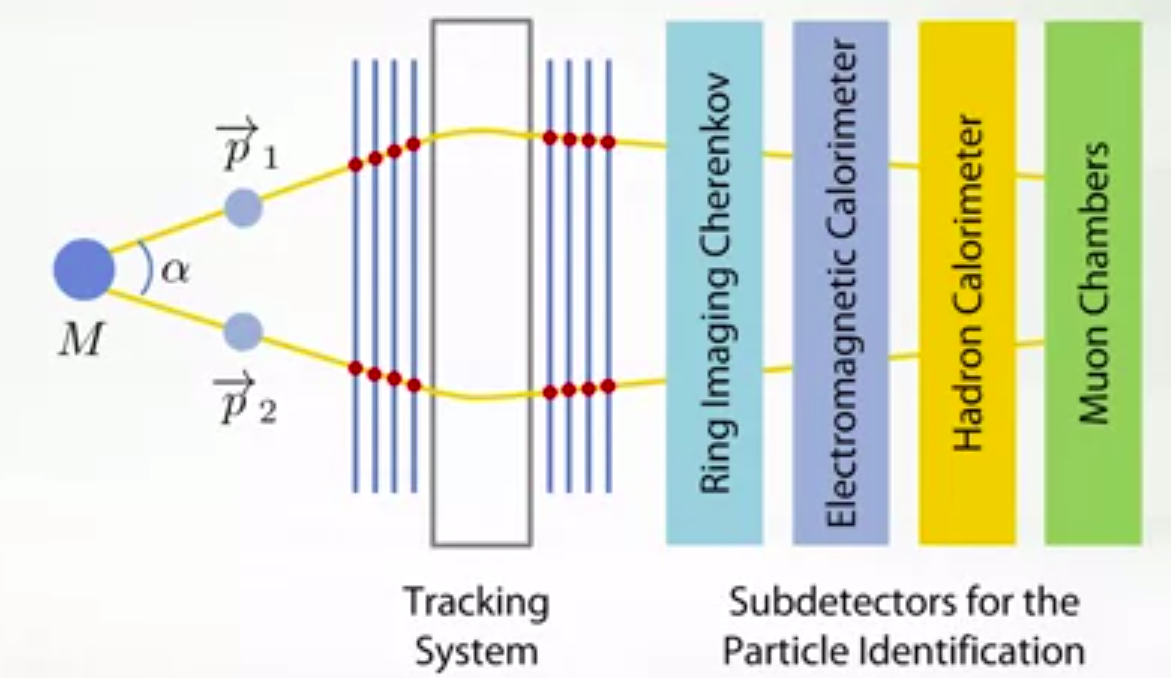
\includegraphics[width=\linewidth]{img/hadron/particleid-detector-setup.png}
    \caption{Detector Setup of the LHC}
    \label{fig:particleid-detector-setup}
  \end{subfigure}
  \begin{subfigure}[b]{0.4\textwidth}
    \centering
    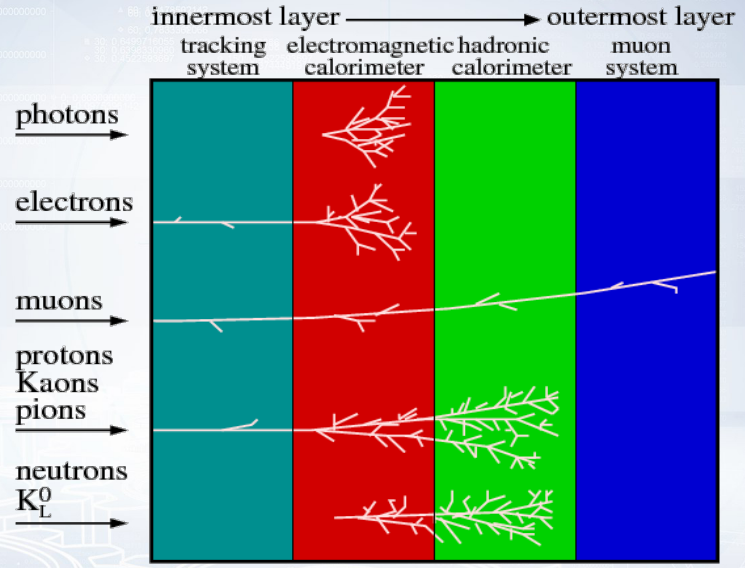
\includegraphics[width=\linewidth]{img/hadron/particleid-tracking.png}
    \caption{The tracks made in the Chambers}
    \label{fig:particleid-tracking}
  \end{subfigure}
\end{figure}


\subsection{Tracking System}

The first system of detectors, stands before particle collision area. Important for parameter estimation. 

There are several layers of sensors that measure hits, and allow us to recognise particle trajectories.
There is also a Magnetic Field that allows us to measure momentum (using radius of curvature in the field).

We have the following conservation equationsm wgeb a particle $D^0$ with mass $m$ breaks into a $K^-$ with mass $m_1$ and a $\pi^+$ with mass $m_2$, and they go away from each other at angle $\alpha$:
\begin{eqnarray}
  E_m &=& E_1 + E_2 \\
  \hat{p_m} &=& \hat{p_1} + \hat{p_2} \\
  E^2 &=& p^2 c^2 + m^2 c^4 \\
  M^2 &=& m_1^2 + m_2^2 + \frac{2}{c^4} (E_1 E_2 - p_1 p_2 c^2 cos\alpha)
\end{eqnarray}

\subsubsection{Problem: Track Pattern Recognition} Recognizing hits that belong to the same track. Currently we have the following methods.
\begin{itemize}
  \item Half Transform and Kalman Filtering. (Statistical, computationally cheaper.)
  \item Hopfield Neural Netorks. (Denby Peterson and Cellular Automaton.)
  \item Convolutional Nerual Networks (classify result as correct or wrong). Recurrent Neural Netorks (predict the next hit location).
\end{itemize}
We can then combine these particle tracks into decays.

\subsection{Ring Imaging Chernekov Detector (RICH)}

This is the first detector because it does not affect the flight of the particle.

\begin{figure}[H]
  \centering
  \begin{subfigure}[b]{0.45\textwidth}
      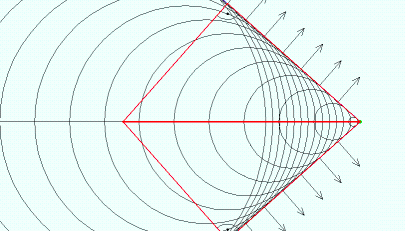
\includegraphics[width=\linewidth]{img/hadron/particleid-chernekov-wavefronts.png}
      \caption{Chernekov Simulation}
      \label{fig:particleid-chernekov-wavefronts}
  \end{subfigure}
  \begin{subfigure}[b]{0.30\textwidth}
      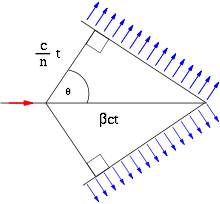
\includegraphics[width=\linewidth]{img/hadron/particleid-cherenkov-angles.png}
      \caption{Chernekov Angles}
      \label{fig:particleid-cherenkov-angles}
  \end{subfigure}
  \begin{subfigure}[b]{0.45\textwidth}
    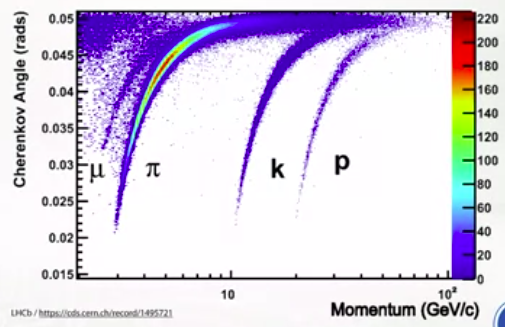
\includegraphics[width=\linewidth]{img/hadron/particleid-chernekov-graph.png}
    \caption{Chernekov Radiation Graphs}
    \label{fig:particleid-cherenkov-angles}
\end{subfigure}
\caption{Registers in Processor Design}
\end{figure}

Here is the angle of the Chernokov radiation, derivable using simple geometric means and some special relativity in terms of the momentum.
\begin{equation}
  p = \frac{mc\beta}{\sqrt{1 - v^2/c^2}}
\end{equation}
\begin{equation}
  cos \theta = \frac{1}{n\beta} = \frac{\sqrt{p^2 + m^2c^2}}{np}
\end{equation}
From the figure above, and the equation for it's analytical feel, that we can figure out the mass of the particle and thereby which particle it is.

% ISSUE: 5:40 Kaon and Pion rings.

\subsection{Ring Imaging Chernekov Detector (RICH)}

Electromagnetic calorimeter - stops everything other than muons and quarks.
Hadron calorimeter - stops the quarks.
\chapter{Quantum Field Theory}



\section{Classical Field Theory}


\subsection{What is a field?}

A field $\phi$ is a quantity (eg. Density, Spin, Charge) defined at every point in a manifold $M$ (spacetime, Minkowski space usually).

\begin{equation*}
  \phi : M \leftarrow S
\end{equation*}
So the field is any function from the space to a Target Space.
\begin{itemize}
  \item Here $S$ can be Scalar Field, where $S = \Re$. It good for modeling Higs Boson, Charge Density, Magnetisation density, etc.
  \item Or it can be a vector field $S = \Re^n$. It's good for modelling Pions, Elecromagnetic fields, etc.
  \item We can also have $S = S^2$, which is the surface of a sphere, this is used for the $\sigma$-model and modelling Quantum Magnets.
\end{itemize}

We will restrict our attention to fields whose Classical Dynamics are obtained by applying Variational Principal applied to an Action Functional (Lagrangian Fields). These encode symetries well.


\subsection{Our Lagrangian Field}

We break our vector field down into several scalar fields, $\Phi_a(x)$; $a = 1,2,3\dots,N$.

Our action functional involves the Lagrange density $\mathcal{L}$ which is a function of 
\begin{equation*}
  S(\Omega) = \int_\Omega \mathcal{L}(\partial_\mu \Phi_a) d^4x\;\;;\;\; d^4x = dx_0 dx_1 dx_2 dx_3.
\end{equation*}
Here $\Omega \in \mu_{1,3}$ is a measurable subset of spacetime, the region where $\mathcal{L}$ is defined.

$\mathcal{L}$ is a function if $\Phi_a$, $\partial_\mu \Phi_a$, $\partial_\mu \partial_\nu \Phi_a$, and so on, but we will only take the first derivative, so:
\begin{equation}
  \mathcal{L} = \mathcal{L}(\Phi_a, \partial_\mu \Phi_a)
\end{equation}
And does not depend on the higher derivatives in space, i.e. $\partial_\mu \partial_\nu \Phi_a$ and so on. NOTE that this is an ASSUMPTION, only due to our needs of nice Lagrangian like equations.

We assume that this functional is stationary under small perturbations, i.e. only the second derivative varies, not till the first derivatives. $\Phi_a(x) \longrightarrow \Phi_a(x) + \delta \Phi_a(x)$. But on the boundary 


\subsection{Extracting Equations of Motion}

The Lagrangian density is essentially a highly compressed representation that contains a lot of equations of motion.
We start by taking a path $\Omega$ and creating a perturbation, and evaluate the change in the Lagrangian.
\begin{eqnarray}
  S[\omega] &=& \int_\omega \mathcal{L}(\Phi, \partial_\mu \Phi) \\
  \delta S &=& \int d^4 x \delta \mathcal{L} \\
           &=& \int d^4x (\frac{\partial \mathcal{L}}{\partial \Phi} \cdot \delta \Phi + \frac{\partial \mathcal{L}}{\partial (\partial_\mu \Phi)} \cdot \delta(\partial_\mu \Phi))
\end{eqnarray}
Now we can integrate by parts, first we have the observation on the second term, we see that it's one of the two terms of a product derivative, so we go for the integral. Then we note that our fields die out on the boundaries of space and time, so the integral falls out to 0, and all we are left with is the generalized Euler-Lagrange equations.
\begin{eqnarray}
  \partial_\mu (\frac{\partial \mathcal{L}}{\partial \partial_\mu \Phi} \cdot \delta \Phi) = \partial_\mu (\frac{\partial \mathcal{L}}{\partial \partial_\mu \Phi} \cdot \delta \Phi) + \partial_\mu (\frac{\partial \mathcal{L}}{\partial \partial_\mu \Phi}) \cdot \delta \Phi
\end{eqnarray}


\begin{equation}
  \frac{\partial \mathcal{L}}{\partial \Phi_a} - \frac{\partial}{\partial x^\mu} \frac{\partial \mathcal{L}}{\partial (\partial_\mu \Phi_a)} = 0
\end{equation}


\subsection{Example: Klein Gordon Field}

This is one of the most general examples of a classical field that is Relativistically invarient.
\begin{equation}
  \mathcal{L} = \frac{1}{2} (\partial_0 \Phi)^2 - \frac{1}{2} (\nabla \Phi)^2 - \frac{1}{2} \mu^2 \Phi^2
\end{equation}

Using Euler-Lagrange on this, we get the following equation of motion:
\begin{equation*}
  \frac{\partial}{\partial x^u} (\partial^\mu \Phi) + m^2 \Phi = 0
\end{equation*}
\begin{equation}
  \Box \Phi + m^2 \Phi = 0
\end{equation}
We note that this is quite similar to the Wave Equation, or the Schrodinger equation, but here in 4-D space.


\subsection{Hamiltonian Formalism}

To guess quantum theories with classical limits determined by $\mathcal{L}$, we want to find the conjugate variables, and then impose canonical commutation relations.
If $\Phi_a(x)$ is "canonical position", then the "conjugate momentum density" is $\pi_a(x) = \frac{\partial \mathcal{L}}{\partial \dot{\Phi_a}}$.



\section{Symetries in Classical Field Theory}


\subsection{What are Symetries}
If $\mathcal{L}(\Phi_a, \partial_\mu \Phi_a)$ is a Lagrange density for some field $\Phi_a(x)$, we consider an infinitesimal transformation:
\begin{equation}
  \Phi_a^\prime(x) = \Phi_a(x) + X_a(\Phi_a)
\end{equation}
Then we have a symmetry if and only if
\begin{equation}
  \mathcal{L} \longrightarrow \mathcal{L}(\Phi_a^\prime, \partial_\mu \Phi_a^\prime) = \mathcal{L}(\Phi_a, \partial_\mu \Phi_a) + \partial_\mu F^\mu
\end{equation}
Since this implies that the equations of motion do not change, as the Euler Largrange density is invarient upto a total derivative in the Lagrangian.

\subsection{Noether's Theorem}
Every continuous symmetry of a Lagrangian implies that the existance of a conserved current $j^\mu(x)$, where:
\begin{equation}
  \partial_\mu j^\mu = 0
\end{equation}

\begin{proof}{Noether's Theorem}
  We add a $\delta \Phi_a$ as an infinitesimal arbitrary change.
  \begin{eqnarray*}
    \delta \mathcal{L}(\Phi_a, \partial_\mu \Phi_a) &=& \mathcal{L}(\Phi_a + \delta \Phi_a, \partial_\mu (\Phi_a + \delta \Phi_a)) - \mathcal{L}(\Phi_a, \partial_\mu \Phi_a) \\
    &=& \frac{\partial \mathcal{L}}{\partial \Phi_a} \delta \Phi_a + \frac{\partial \mathcal{L}}{\partial \partial_\mu \Phi_a} \delta \partial_\mu \Phi_a
  \end{eqnarray*}
  \danger
  But we also know, for conservation laws,
  \begin{eqnarray*}
    \delta \mathcal{L} = \partial_\mu F^\mu \\
    \partial_\mu (\frac{\partial \mathcal{L}}{\partial \partial_\mu \Phi_a} X[\Phi_a] - F^\mu) = 0
  \end{eqnarray*}
And here we have the conserved current that we were looking for, in the brackets, and we see it's derivative evaluates to 0.
\end{proof}

This also defines the law of conserved charge, since current density vanishes fast till $\infty$, and when we take all of space we have the conservation law.

We feel that every classical symmetry should have a corresponding quantum symetries, this is because the quantum theories must exhibit those symetries in the classical symetries. Also, these charges can help us derive those symmetries.


\subsection{Examples}

\subsubsection{Spacetime Translations}
% What is active transformation
We consider the active transformation $x^\mu \rightarrow x^\mu - \epsilon^\mu$.

This gives us 4 symetries, which is 4 conserved currents, which gives us 16 numbers in total. % Why 16 numbers.
We get the Energy-Momentum (Stress-Energy) tensor, each column of which corresponds to a conserved current.







\section{Theory Reading}

We think of Lagrangian as a function of time, $\mathcal{L}(t)$, and so we call the Lagrangian dependent on the space, i.e. defined on every point in space as the Lagrangian Density. When we integrate it over space, we call it the Lagrangian. Similarly for the Hamiltonian and the Hamiltonian density.

\begin{definition}{}
  \begin{equation}
  \phi \in \mathbb{C}^2 (\mathcal{M}, S)
  \end{equation}
  This means that $\phi$ is twice differentiable in Complex numbers, and a function from $\mathcal{M}$, the minkowski space, and S is our target space.
\end{definition}

Also note the following, this is what Covarient and Contravarient derivatives mean, specially as in the Klein Gordon equation.
\begin{equation}
  \partial_\mu \partial^\nu = \eta^{\mu \nu} \partial_\mu \partial^\nu
\end{equation}



\section{Quantizing the Field}


\subsection{Motivation}

We are trying to discover Quantum Theories, loosely defined by a Hilbert Space and a Hamiltonian. Mutiple Quantum Theories can correspond to the same Classical Limit, so Quantizing is an Educated Model. If Hamiltonian $\mathcal{H}$ is only dependent upon coordinates and their squares

\begin{eqnarray}
  (q_j, p_j) &\longrightarrow& (\hat{q_j}, \hat{p_j}) \\
  \delta_{j, k} = \{p_j, q_k\}_{j, k} &\longrightarrow& [p_j, q_k] = i \delta_{j, k} \\
  H &\longrightarrow& \hat{H} = \sum_{k} \frac{p_j^2}{2m} + \frac{m}{2} \sum_{j, k} q_j [Q]_{jk} q_k \\
\end{eqnarray}

\subsection{Solving for Hamiltonian}

We know that there exists a diagonalizing orthogonal matrix O, such that $OO^T = \mathbb{I}$. Let this have our $\omega^2$s as it's eigen values, since it's the energy eigenvalues.
\begin{equation}
  O Q O^T = \begin{bmatrix}
    \omega_1^2 & 0 & 0 & ...\\
    0 & \omega_2^2 & 0 & ... \\
    0 & 0 & \omega_3^2 & ... \\
    ... & ... & ... & ...
  \end{bmatrix}
\end{equation}

We take the following relations and substituite into the hamiltonian to get the hamiltonian in the new coordinates.
\begin{eqnarray}
  \hat{q_j^\prime} &=& \sum_{k=1}^n [O]_{jk} \hat{q_k} \\
  \hat{p_j^\prime} &=& \sum_{k=1}^n [O]_{jk} \hat{q_k}
\end{eqnarray}

We get the following Hamiltonian, we can quanitize it (diagonalize it) by constucting the Creator and Annahiator operators.
\begin{equation}
  \hat{H} = \sum_{j=1}^n \frac{p_j^2}{2m} + \frac{1}{2} m \sum_{l=1}^{n} \omega_l^2 \hat{q_l^\prime}^2
\end{equation}



\section{Commutation Relations}

\begin{equation}
  [\Phi_a(x), \Pi^b(y)] = i \delta^{(3)}(\vec{x} - \vec{y}) \delta^b_a
\end{equation}



\chapter{General Relativity}



\section{Preliminaries}


\subsection{What is flat space}

Space is flat if there exists a way to chose the metric tensor, such that it's the knonecker delta. $\eta^{x,y} = \delta_{x,y}$.

\begin{small}
  A piece of flat paper that is folded is still flat, it has no curvature, it can be made flat again and the notion of distance is still the same as when it was flat. This is just extrinsic curvature, which comes from the way it's embedded in a higher dimentional space.
\end{small}


\subsection{Tensor Analysis}

\paragraph{} When we take the components as scalar that sum to it, the components are contravarient components.
\begin{equation}
  V = V^1 \hat{e}_1 + V^2 \hat{e}_2 + V^3 \hat{e}_3
\end{equation}

And if we find the components using dot products, we get the covarient components.
\begin{equation}
  V_n = V \cdot \hat{e}_n = \Sigma_n V^n (e_n \cdot e_m)
\end{equation}

These are exactly the same thing when we are in the Cartesian coordinates.

\subsubsection{Transformation Rules of Tensors}

\paragraph{} For contravarient index:
\begin{equation}
  dy^m = \frac{\partial y^m}{\partial x^n} dx^n
\end{equation}
\begin{equation}
  \frac{\partial S}{\partial y^m} = \frac{\partial x^n}{\partial y^m} \frac{\partial S}{\partial x^n}
\end{equation}

\paragraph{} For covarient index:
\begin{equation}
  dy^m = \frac{\partial y^m}{\partial x^n} dx^n
\end{equation}
\begin{equation}
  \frac{\partial S}{\partial y^m} = \frac{\partial x^n}{\partial y^m} \frac{\partial S}{\partial x^n}
\end{equation}

\paragraph{} For Mixed tensors (Rank 2):
\begin{equation}
  (W^\prime)^m_n = \frac{\partial y^m}{\partial x^p} \frac{\partial x^q}{\partial y^n} W^p_q
\end{equation}
\paragraph{} For Covarient tensors (Rank 2):
\begin{equation}
  (W^\prime)_{mn} = \frac{\partial x^p}{\partial y^m} \frac{\partial x^q}{\partial y^n} W_{pq}
\end{equation}
\paragraph{} For contravarient tensors (Rank 2):
\begin{equation}
  (W^\prime)^{mn} = \frac{\partial y^m}{\partial x^p} \frac{\partial y^n}{\partial x^q} W^{pq}
\end{equation}

\subsubsection{Addition, Multiplication, Contraction}

\paragraph{} We only add tensor if they have indices of the same kind, that is:
\begin{equation}
  T^{m_1,m_2...m_k}_{n_1,n_2...n_l} + S^{m_1,m_2...m_k}_{n_1,n_2...n_l} = (T + S)^{m_1,m_2...m_k}_{n_1,n_2...n_l}
\end{equation}

\paragraph{} We can multiply any two tensors (We do get tensors of higher rank):
\begin{eqnarray}
  V^m \otimes W_n &=& X^m_n  \\
  V^m \otimes W^n &=& X^{mn} \\
  V_m \otimes W_n &=& X_{mn}
\end{eqnarray}

\paragraph{} The generalization of inner product of two vectors to tensors is called it's contraction.
Proof/Intuition of contraction:
\begin{equation}
  (V^m W_m)^\prime = \frac{\partial }{\partial} (V^a W_b)
\end{equation}
\paragraph{} When we contract an upper with a lower index, we reduce the number of indices (rank) by 2, as both of them become dummy indices, and we sum over them.

\subsubsection{The Metric Tensor}

\begin{equation}
  ds^2 = g(x)_{mn} dx^m dx^n
\end{equation}
\paragraph{} The metric tensor is always symetric. Everyone agrees on the length of every vector, though not on the individual components, when viewed from different frames.

Transformation of the metric tensor:
\begin{equation}
  g_{mn}(x) dx^m dx^n = g_{pq}^\prime dy^p dy^q = g_{mn}(x) = \mathbf{g_{pq} \frac{\partial x^m}{\partial x^n} \frac{\partial y^p}{\partial y^q}} dy^p dy^q
\end{equation}

\paragraph{} We have two metric tensors, one with covarient and one with contravarient indices, defined as:
\begin{equation}
  g_{mn} g^{np} = \delta_m^p
\end{equation}
So, one is the inverse of the other.



\section{Cartesian Geometry}


\subsection{Flatness of a Space}

If $g_mn \neq \delta_mn$ (metric tensor), this does not mean that the space is flat. This just means we have bad coordinates. Let's say there is some quantity Riemann $R$.

In Riemannian Geometry, all lengths are positive, all of their squares are also positive. Equivalently, the metric tensor is positive definite, i.e. all it's eigen values are positive.


\subsection{Gaussian Normal Coordinates}

At every point, we can chose Gaussian Normal Coordinates (unique upto all rotations), such that $g_{mn} = \delta_{mn}$ at $r = r_0$. Also we can chose $\frac{\partial g_{mn}}{\partial x^r} = 0$, i.e. our metric can be chosen to have first derivative 0. We can only make higher derivatives 0 iff the space is flat, but not otherwise $\frac{\partial^2 g_{mn}}{\partial x^r \partial x^s} \neq 0$.

This can always be done since $x^m = y^m + c^m_{nr} y^n y^r$ is the most general quadratic, and it contains 40 free constants in 4-spaces, since all of $c^m_{nr}$ are all free. But this only allows us to set the derivatives of all 10 variables to 0 with respect to each of the 4 variables, so we have derivative to first order is 0.

\textbf{The meeaning of Covartient derivatives is that they are all 0 in Gaussian Normal Coordinates, and then making Tensors out of them}.
\begin{eqnarray}
  D_s g_mn &=& \frac{\partial g_mn}{\partial x^s} - \Gamma^{t}_{sm} g_{tn} - \Gamma^{t}_{sn} g_{mt} = 0 \\
  D_m g_sn &=& \frac{\partial g_sn}{\partial x^m} - \Gamma^{t}_{sm} g_{tn} - \Gamma^{t}_{mn} g_{st} = 0 \\
  D_n g_sm &=& \frac{\partial g_sm}{\partial x^n} - \Gamma^{t}_{sn} g_{tm} - \Gamma^{t}_{mn} g_{st} = 0 \\
  \Gamma^{t}_{mn} &=& \frac{1}{2} [\partial_n g_{sm} + \partial_m g_{sn} + \partial_s g_{mn}]
\end{eqnarray}
We got the last equation from (1) + (2) - (3), and so we have the value of the Cristophel symbols. They can be 0 in one frame and non-zero in another, so we go back to the tensor frame after doing the derivatives.



\section{Starting off with Gravitation}

\begin{equation}
  D_M V^n = \frac{\partial V^n}{\partial x^m} + \Gamma_{mn}^{r} V^r
\end{equation}

\end{document}
